%%% Local Variables: 
%%% mode: latex
%%% TeX-master: t
%%% End: 
\documentclass{article}
\usepackage{../tex/mysty}
\begin{document}

\maketitlepage{Societal Impact Report}{Ginger Tsai}

\setcounter{tocdepth}{2}
\tableofcontents
\newpage
\listoftables
\listoffigures
\newpage


\section*{Executive Summary}
\label{sec:exec-summary}

% TODO: Ginger's section


\newpage


\section{Introduction}
\label{sec:introduction}

% TODO: Ginger's section


\section{Notable Concerns}
\label{sec:concerns}

% Introductory sentence (Ginger)


\subsection{Joe's Blah blah blah}
\label{sec:blah-blah-blah}

\subsection{Joe's Blah blah blah}
\label{sec:blah-blah-blah}

\subsection{Sanjay's Blah blah blah}
\label{sec:blah-blah-blah}

\subsection{Sanjay's Blah blah blah}
\label{sec:blah-blah-blah}

\subsection{Shuyen's Demographic}
\label{sec:Demographic}
	The design solution (3D imaging device) is targeted at....
\subsection{Shuyen's Public Policy}
\label{sec:Public Policy}
	The design solution will not be regulated by the FDA ....
\section{Conclusion}
\label{sec:conclusion}

% TODO: Ginger's section

\section{Addendums}
\label{sec:addendums}

\subsection{Tables}
\label{sec:tables}

\begin{table}[H]
  \footnotesize
  \centering
  \begin{tabularx}{\textwidth}{llXX}
    \toprule
    \textbf{Type} & \textbf{Specification} & \textbf{Metric} & \textbf{Justification} \\
    \hline
    Need & Resolution & 2 micron & Choice of scan pattern \\
    Need & Speed & 1 scan within 3 minutes & Choice of scan pattern and drive \\
    Need & 3D image reconstruction & None & Choice of scan pattern \\
    Need & Size & 0.75 by 1m footprint (\textit{or:} fits in 0.75m $\times$ 1m $\times$ 1m space) & Internal compartment design \\
    Need & Electrical Properties & 120V 60Hz AC & Choice of material \\
    Need & Thermal Properties & Functions in $22\pm5$ °C & Choice of material \\
    Need & Chemical Properties & Withstand $<1$ mL of PBS & Choice of material \\
    Need & Robustness & Withstand a drop of 3 feet, sudden sideways movement & Internal compartment design, choice of material \\
    Want & Weight & $<40$ lbs (18 kg) & Internal compartment design, choice of material \\
    Want & User Interface & Requires 1 click of the mouse for measurement transfer from device to computer & Software design \\
    Want & Reusable & Up to 4 years given use of $5^+$ times/day, 1 hour per use & Internal compartment design, choice of material \\
    Want & Minimize vibration & N/A & Component properties \\
    Want & Simplicity & Few hanging, external components; manageable design & External design \\
    Want & Cost & Manufacturing cost $<\$10,000$ & Internal and external design, choice of material \\
    Desire & Aesthetics & Aesthetically pleasing, easy on the eyes & External design, choice of material \\
    Desire & Noise & $<80$ dB & Internal compartment design, choice of material \\
    \bottomrule
  \end{tabularx}
  \figcaption{
    \textbf{Engineering Design Specifications:}
  This is the detailed list of engineering design specifications, categorized by priority in terms of ``need'', ``want'', or ``desire''.}
  \label{tab:eds}
\end{table}

\begin{table}[H]
  \footnotesize
  \centering
  \begin{tabularx}{\textwidth}{XcXX}
    \toprule
    \textbf{Item} & \textbf{Price} & \textbf{Function} & \textbf{Supplier} \\
    \hline
    Keyence LED micrometer                                          & ---      & obtains measurements of eye dimensions                            & adviser - Dr John Nickerson                    \\
    LabVIEW Development System 8.6                                  & ---      & reconstructs and interprets data from micrometer                  & Georgia Tech Biomedical Engineering department \\
    Stanley GR10 Mini Hot Melt Glue Gun                             & \$3.99   & simulates optic nerve                                             & Sears                                          \\
    Stanley 12-Pack All purpose-4" Clear Miniature Glue Sticks      & \$2.00   & simulates optic nerve (in conjunction with hot glue gun)          & thehardwarecity.com (online)                   \\
    plastic ABS mold                                                & ---      & simulates an eyeball                                              & Georgia Tech Biomedical Engineering department \\
    Oral-B Mint Ultra Floss, 1 count, 2 pack                        & \$4.00   & simulates optic nerve (with plastic eyeball)                      & Wal-Mart                                       \\
    Koji eyebrow tweezers                                           & ---      & holds simulated eyeball; simulates tweezer action on optic nerve  & group member                                   \\
    Irwin Quick-Grips                                               & ---      & holds and controls tweezers                                       & Georgia Tech Biomedical Engineering department \\
    Rotational motor                                                & ---      & rotates eyeball                                                   & Georgia Tech Biomedical Engineering department \\
    Firgelli Automations 6" stroke 8lbs Force Linear Actuator 12V   & \$75.00  & vertically translates micrometer and micrometer platform          & robotshop.us (online)                          \\
    Linear Encoder                                                  & \$100.00 & determines position of micrometer                                 & online       \\
    Microscope Stage                                                & \$80.00  & serves as platform upon which micrometer will stand               & online                                  \\
    Wiring                                                          & ---      & connects motors and drives to micrometer and clamp/tweezer system & Georgia Tech Biomedical Engineering department \\
    \hline
    \textbf{Total} & \$345 & & \\
    \bottomrule
  \end{tabularx}
  \figcaption{
    \textbf{Budget for Developing the Prototype:}
  Each component of the prototype is listed along with price, function, and supplier. Blank prices indicate that the component is being provided for free. The final price estimate is lower than the actual anticipated cost as the budget doesn't account for contingencies.}
  \label{tab:expenses}
\end{table}

\subsection{Figures}
\label{sec:figures}

\begin{figure}[H]
  \centering
  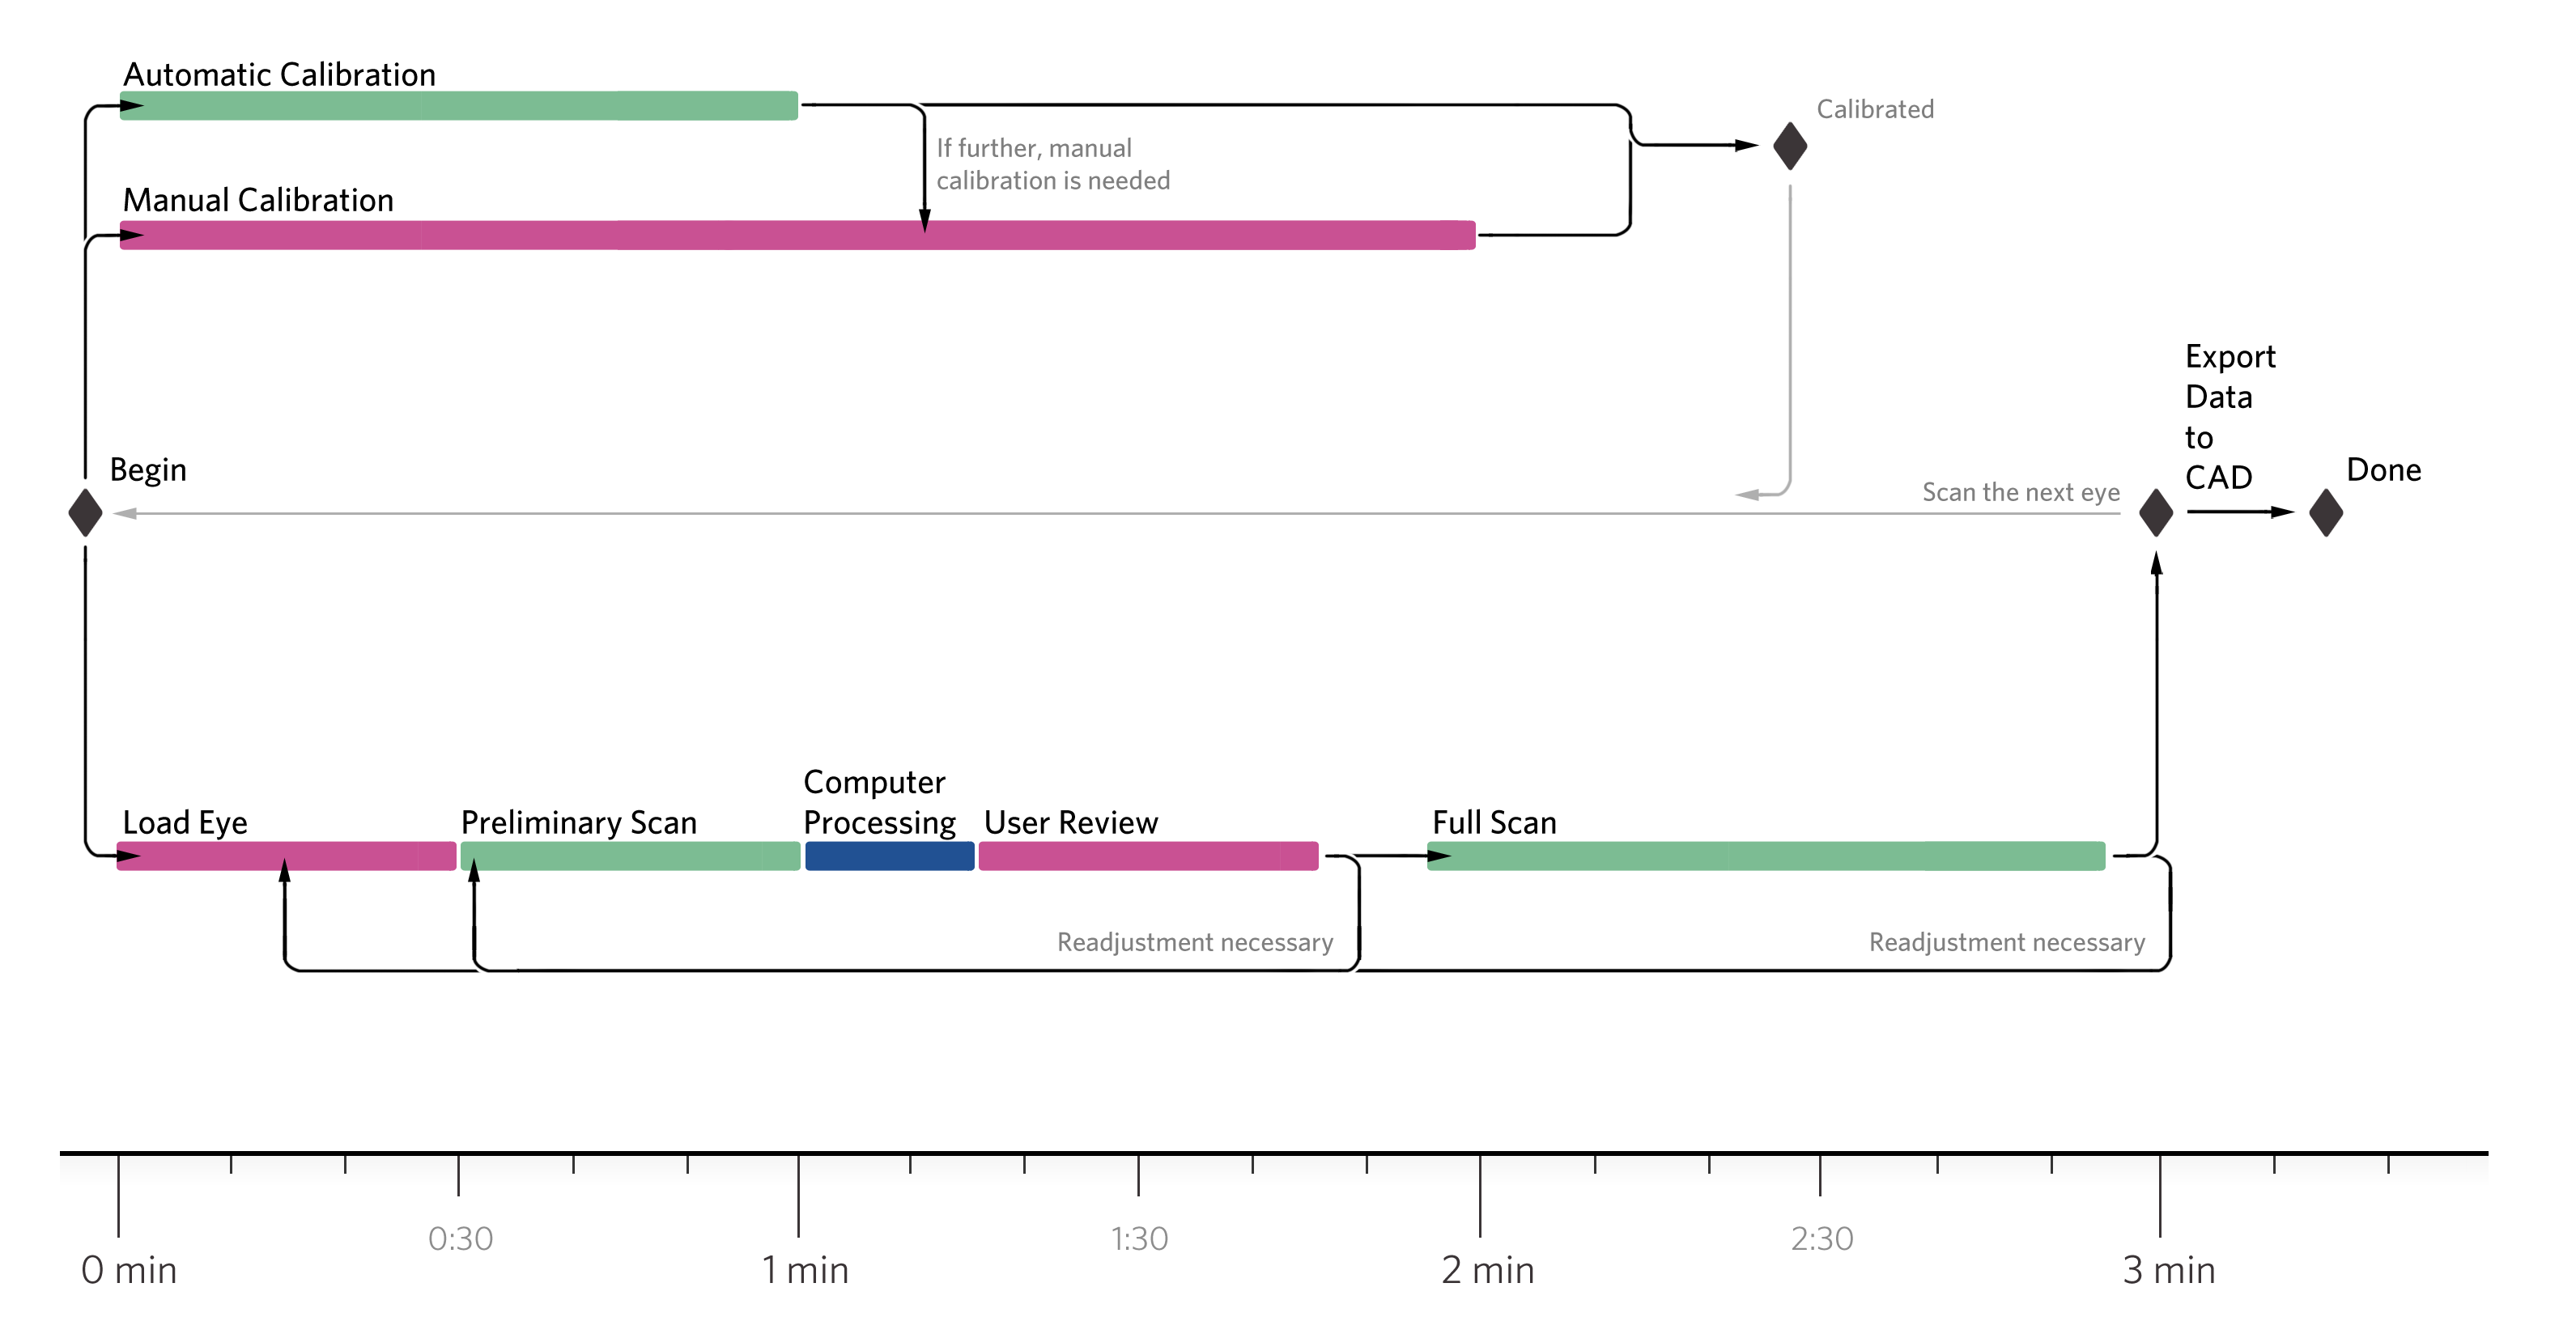
\includegraphics[width=\linewidth]{../img/usage_flow}
  \figcaption{\textbf{Possible Usage Flowchart:}  
  The device is controlled via the computer interface in order to perform a number of tasks required for repeatable, accurate measurement of an eye. Each task is located at and extended over the suggested period of time required to perform the task. Colors of the task boxes encode the required user interaction. Red tasks require direct user interaction with the physical harness, green tasks only require interaction with the computer, and blue tasks are computational tasks where the user must wait.}
  \label{fig:usage}
\end{figure}

\begin{figure}[H]
  \centering
  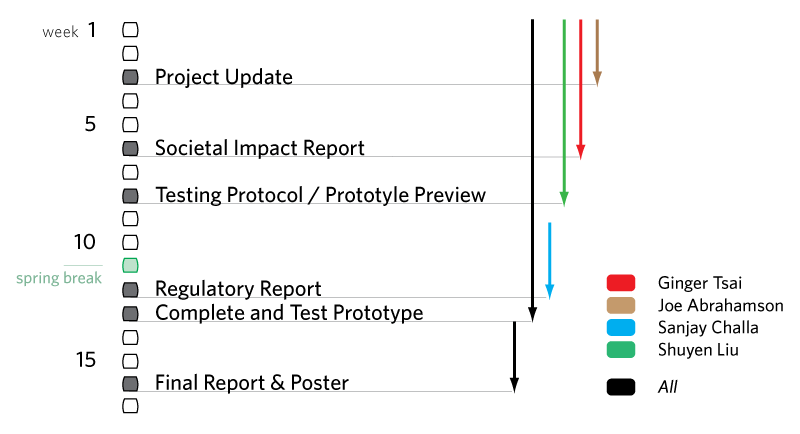
\includegraphics[width=0.75\linewidth]{../img/spring_gantt}
  \figcaption{\textbf{Gantt Chart:}
  The arrows are color coded indicating the primary author of each document. Tasks, duration of tasks, and milestones are clearly illustrated by the arrows and corresponding text at the head of each arrow.}
  \label{fig:gantt}
\end{figure}

\begin{figure}[H]
  \centering
  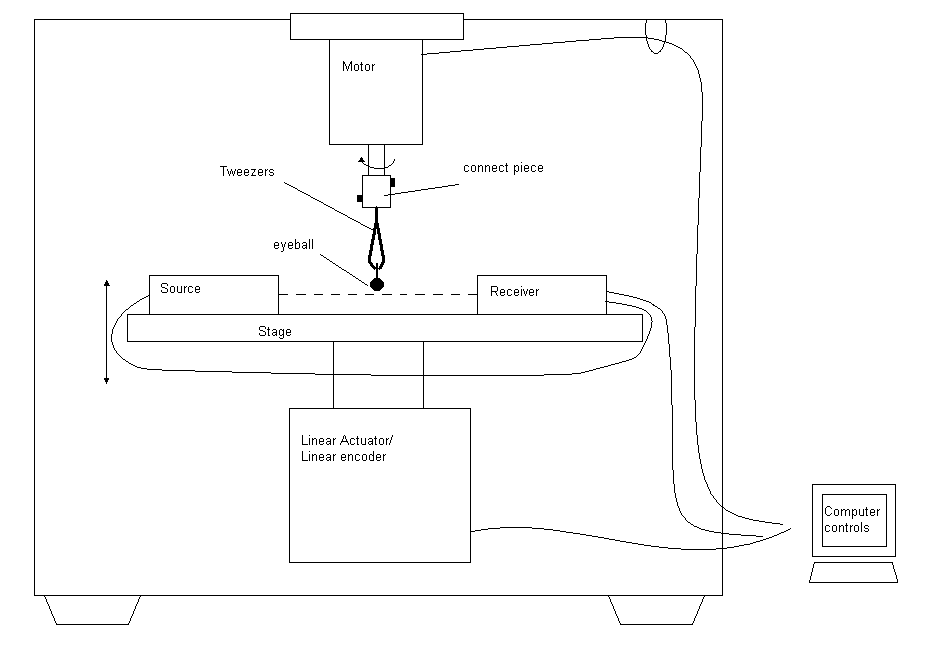
\includegraphics[width=\linewidth]{../img/schematic1}
  \figcaption{\textbf{Schematic of the Prototype:}  
  This figure illustrates the physical organization of the various components of the design within an enclosed framework. Each component is labeled. }
  \label{fig:schematic1}
\end{figure}

\newpage
\addcontentsline{toc}{section}{References}
\bibliographystyle{unsrt}
\bibliography{../tex/bibl}

\end{document}
